% !TEX TS-program = pdflatexmk

\documentclass[14pt]{beamer}
\usepackage{newtxtext,newtxmath}
\usepackage{microtype}
\usepackage[english]{babel}
\usepackage{hyperref}
\usepackage{graphicx}
\usepackage{listings}
\lstloadlanguages{Python}
\lstset{language=Python}
\lstset{%
basicstyle=\ttfamily\bfseries,
keywordstyle=\color{blue}, emph={self}, emphstyle={\color{blue}},
identifierstyle=,
commentstyle=\color{brown},
stringstyle=\color{green!50!black},
showstringspaces=false,
emphstyle={[2]\color{purple}},
}
\usepackage{tikz}
\usepackage{forest}
\usetikzlibrary{positioning}
\usepackage{array}
\newcolumntype{L}[1]{>{\raggedright\let\newline\\\arraybackslash\hspace{0pt}}m{#1}}

\mode<presentation>{
\usetheme{Madrid}
\definecolor{uabgreen}{cmyk}{.89,.31,.78,.17}
\usecolortheme[named=uabgreen]{structure}
\setbeamertemplate{navigation symbols}{}
\setbeamertemplate{footline}[frame number]
\setbeamertemplate{section in toc}[square]
\setbeamertemplate{subsection in toc}[square]
\setbeamertemplate{items}[square]
\setbeamercovered{transparent=5}
}

\newcommand{\keyword}[1]{{\color{blue}#1}}
\newcommand{\cmnt}[1]{{\color{gray}#1}}
\newcommand{\str}[1]{{\color{green!50!black}#1}}
\newcommand{\defn}[1]{{\color{purple}#1}}

\author[Dr. Bethard]{Dr. Steven Bethard}
\institute[UAB CIS]{%
Computer and Information Sciences\\
University of Alabama at Birmingham}

\AtBeginSection[]
{
  \begin{frame}<beamer>{Outline}
    \tableofcontents[currentsection]
  \end{frame}
}

\tikzset{
  invisible/.style={opacity=0,text opacity=0},
  visible on/.code={%
    \alt<#1>{}{\pgfkeysalso{invisible}}
  },
  filled on/.code={%
    \alt<#1>{\pgfkeysalso{fill=gray}}{}
  },
}
\forestset{
  edge weight/.style={
    edge label={node[midway,above,sloped]{#1}}},
  invisible/.style={
    /tikz/invisible,
    edge={/tikz/invisible}},
  visible on filled on/.code n args={2}{%
    \alt<#1>{\alt<#2>{\pgfkeysalso{fill=gray}}{}}{\pgfkeysalso{invisible}}
  },
  visible on/.code={%
    \alt<#1>{}{\pgfkeysalso{invisible}}
  },
}

\lstset{emph={[2]__init__,__str__,hill_climb,simulated_annealing,DealerAgent,take_action}}

\newcommand{\searchstate}[1]{\mbox{\texttt{\bfseries\color{red}#1}}}
\newcommand{\searchaction}[1]{\mbox{\textsc{\bfseries\color{red}#1}}}


\title{Beyond Classical Search}
\date[]{16 Jan 2014}

\begin{document}

\begin{frame}
  \titlepage
\end{frame}

\begin{frame}{Outline}
  \tableofcontents
\end{frame}

\section{Local Search}
\begin{frame}{Local Search}
	\begin{block}{Sometimes only the goal matters (not the path)}
		\begin{itemize}
			\item 8-Queens
			\item Bag Generation
			\item Job Scheduling
		\end{itemize}
	\end{block}
	\begin{block}<2->{Iterative Improvement}
		Single \textit{current} state, explores neighbors
		\\ \medskip
		\begin{tabular}{ll}
			\uncover<3->{Memory?}   & \uncover<4->{$O(1)$} \\
			\uncover<5->{Optimal?}  & \uncover<6->{\textit{Usually not}} \\
			\uncover<7->{Complete?} & \uncover<8->{\textit{Usually not}} \\
		\end{tabular}
	\end{block}
\end{frame}
\begin{frame}{Example: Travelling Salesperson Problem}
	\begin{block}{Problem}
		Visit all cities exactly once, minimum distance
	\end{block}
	\begin{description}
		\item[Start] A random complete tour
		\item[Move] Swap a pair to reduce total distance
	\end{description}
	\begin{center}
		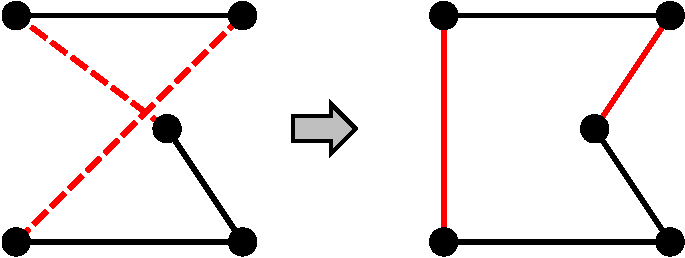
\includegraphics[height=1in]{tsp-sequence.pdf}
	\end{center}
	Achieves 1\% of optimal with thousands of cities
\end{frame}
\begin{frame}{Example: $n$-queens}
	\begin{block}{Problem}
		Put $n$ queens on an $n \times n$ board \\
		No two queens	on the same row, column, or diagonal
	\end{block}
	\begin{description}
		\item[Start] All queens placed randomly
		\item[Move] Move a queen to reduce conflicts
	\end{description}
	\begin{center}
		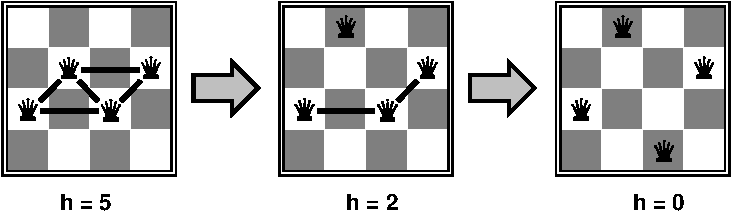
\includegraphics[height=1in]{4-queens-iterative.pdf}
	\end{center}
	Can solve $n$-queens problems for, e.g. $n = 1$ million
\end{frame}

\subsection{Hill Climbing}
\begin{frame}[fragile]{Hill Climbing}
	\scriptsize
	\begin{lstlisting}
		def hill_climb(problem):
		
		    # start at the problem's initial state
		    current = Node(problem.get_random_complete_state())
		    while True:
		
		        # select the neighboring state with the best score
		        state_scores = []
		        for state, score in problem.get_neighbors(current.state):
		            state_scores.append((score, state))
		        best_score, best_state = max(state_scores)
		
		        # if no neighbors are better, return the current
		        if best_score <= current.score:
		            return current.state
		
		        # otherwise, move current to the best state
		        current = Node(best_state, best_score)
	\end{lstlisting}
\end{frame}
\begin{frame}{Hill Climbing}
	\begin{center}
		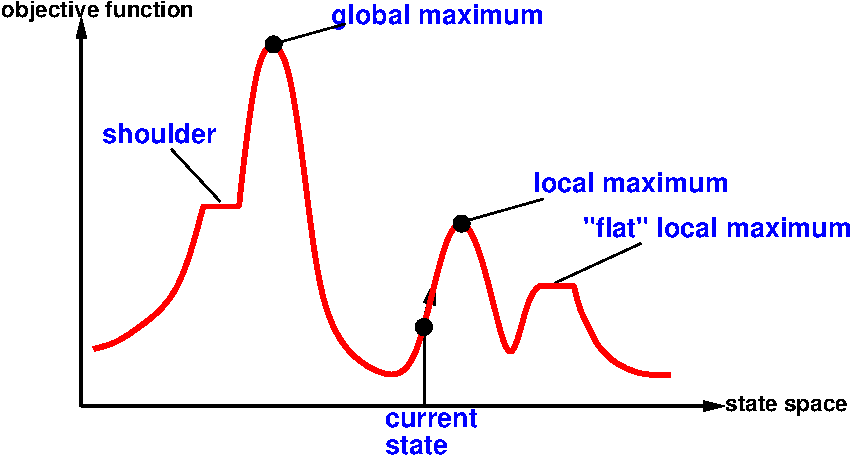
\includegraphics[width=4in]{hill-climbing.pdf}
	\end{center}
\end{frame}

\subsection{Random Hill Climbing}
\begin{frame}{Un-Sticking Hill Climbing}
	\begin{block}{Sideways Moves}
		Allow moving to neighbors as good as the current
	\end{block}
	\begin{block}<2->{Stochastic Hill Climbing}
		Choose randomly from \textit{all} neighbors that improve score
	\end{block}
	\begin{block}<3->{Random Restart Hill Climbing}
		Generate a new initial state and try again \uncover<4->{\alert<4->{Complete!}}
	\end{block}
	\begin{block}<5->{Simulated Annealing}
		Some bad moves; gradually decrease size and frequency \\
		\uncover<6->{\alert<6->{Complete and Optimal if ``gradual'' enough}}
	\end{block}
\end{frame}
\begin{frame}[fragile]{Simulated Annealing}
	\scriptsize
	\begin{lstlisting}
		def simulated_annealing(problem, get_temperature):
		    current = Node(problem.get_random_complete_state())
		    for time in itertools.count():
		        
		        # stop when the temperature reaches zero
		        temperature = get_temperature(time)
		        if temperature == 0:
		            return current
		        
		        # select a random neighbor
		        neighbors = problem.get_neighbors(current.state)
		        state, score = random.choice(neighbors)
		        
		        # always move to the neighbor if it's better,
		        # and sometimes if it's worse
		        change = score - current.score
		        prob = math.exp(change / temperature)
		        if change > 0 or random.random() < prob:
		            current = Node(state, score)
	\end{lstlisting}
\end{frame}

\subsection{Local Beam Search}
\begin{frame}{Local Beam Search}
	\begin{block}{Idea}
		Keep $k$ states instead of just one
	\end{block}
	\begin{block}<2->{vs. $k$ Random Restarts}
		\uncover<3->{
		One state has good neigbors, others have bad neighbors
		\begin{description}
			\item[Local Beam Search] All searches share good neighbors
			\item[$k$ Random Restarts] Other searches use bad neighbors
		\end{description}
		}
	\end{block}
	\begin{block}<4->{Variants}
		\begin{itemize}
			\item<5-> Keep $k$ best states
			\item<6-> Keep $k$ random states, probabilities based on scores
		\end{itemize}
	\end{block}
\end{frame}
\begin{frame}[fragile]{Local Beam Search}
	\scriptsize
	\begin{lstlisting}
		def local_beam_search(problem, k):
		    current = [Node(problem.get_random_complete_state())]
		    while True:
		        
		        # get all neighbors of the current states
		        state_scores = []
		        for node in current:
		            for state, score in problem.get_neighbors(node.state):
		                
		                # return the first goal state generated
		                if problem.is_goal(state):
		                    return state
		                state_scores.append((score, state))
		        
		        # select the k best states to consider next time
		        current = []
		        for score, state in heapq.nlargest(k, state_scores):
		            current.append(Node(state, score))
	\end{lstlisting}
\end{frame}
\begin{frame}{Genetic Algorithms}
	\begin{block}{Idea}
		\begin{itemize}
			\item Stochastic local beam search
			\item Successors generated from \textbf{pairs} of states
		\end{itemize}
	\end{block}
	\begin{center}
		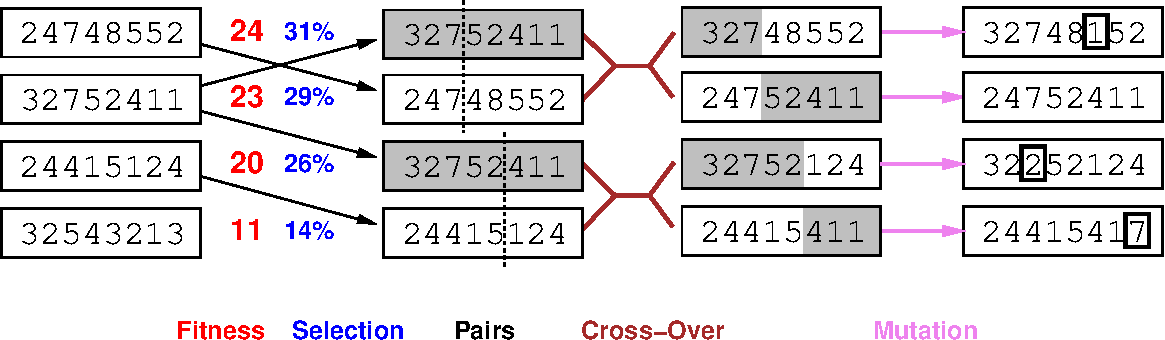
\includegraphics[width=4in]{genetic.pdf}
	\end{center}
\end{frame}
\begin{frame}{Genetic Algorithms}
	\begin{block}{Requirements}
		\begin{itemize}
			\item States must be encoded as strings
			\item Substrings must be meaningful components \\
			      \uncover<2->{\alert<2->{or crossover is pointless!}}
		\end{itemize}
	\end{block}
	\begin{center}
		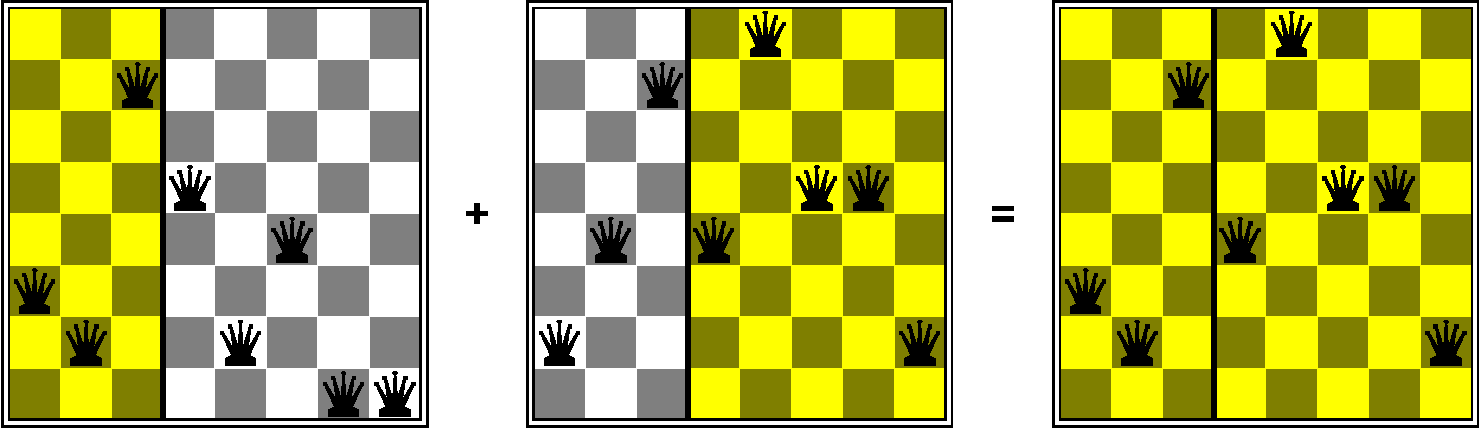
\includegraphics[width=4in]{8-queens-crossover.pdf}
	\end{center}
\end{frame}

\section{Advanced Search}

\subsection{Continuous Search Spaces}
\begin{frame}{Continuous Search Spaces}
	\begin{block}{Problem}
		Place 3 airports in Romania, minimizing
		$\sum\limits_{a \in \mbox{\textit{\scriptsize airports}}}
		 {\sum\limits_{c \in \mbox{\textit{\scriptsize cities}}}
		  {(x_c - x_a)^2 + (y_c - y_a)^2}}$
	\end{block}
	\begin{block}<2->{As a Search Problem?}
		\uncover<3->{
		But there are $\infty$ actions from each state!
		}
	\end{block}
	\begin{block}<4->{Solutions}
		\begin{description}
			\item[Discretize] each action moves $\pm\delta$ in $x$ or $y$ direction
			\item[Gradient] each action moves $\alpha\nabla f(x)$
		\end{description}
	\end{block}
\end{frame}

\subsection{Partial Information}
\begin{frame}{Searching with Partial Information}
	\begin{columns}
		\column{.50\textwidth}
			\begin{block}{Problem}
				Start in \alert{any state}
			\end{block}
			\begin{block}{Solution?}
				\footnotesize
				\begin{tabular}{ll}
					\uncover<2->{Initial}     & \uncover<2->{$\{\searchstate{1}, \searchstate{2}, \searchstate{3}, \searchstate{4}, \searchstate{5}, \searchstate{6}, \searchstate{7}, \searchstate{8}\}$} \\
					\uncover<3->{\searchaction{Right}} & \uncover<4->{$\{\searchstate{2}, \searchstate{4}, \searchstate{6}, \searchstate{8}\}$} \\
					\uncover<5->{\searchaction{Suck}}  & \uncover<6->{$\{\searchstate{4}, \searchstate{8}\}$} \\
					\uncover<7->{\searchaction{Left}}  & \uncover<8->{$\{\searchstate{3}, \searchstate{7}\}$} \\
					\uncover<9->{\searchaction{Suck}}  & \uncover<10->{$\{\searchstate{7}\}$} \\
				\end{tabular}
			\end{block}
		\column{.50\textwidth}
			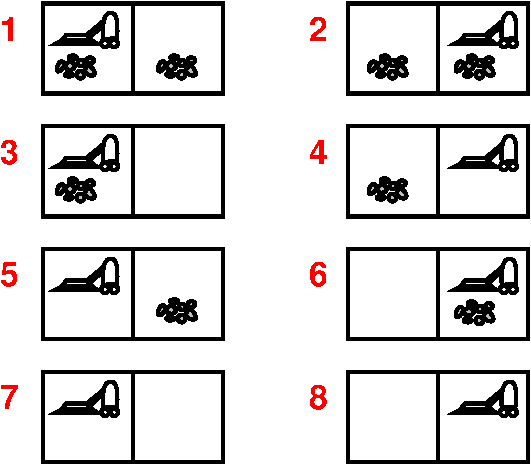
\includegraphics[width=2.1in]{vacuum-space.pdf}
	\end{columns}
\end{frame}

\subsection{Online Search}
\begin{frame}[label=real-time-astar]{Online Search}
\begin{block}{Problem}
Successor function is not available until a state is visited, \\
e.g. robot exploration, maze problems
\end{block}
\begin{block}<2->{Solution: Learning Real-Time A*}
Augment hill climbing with memory
\begin{center}
\footnotesize
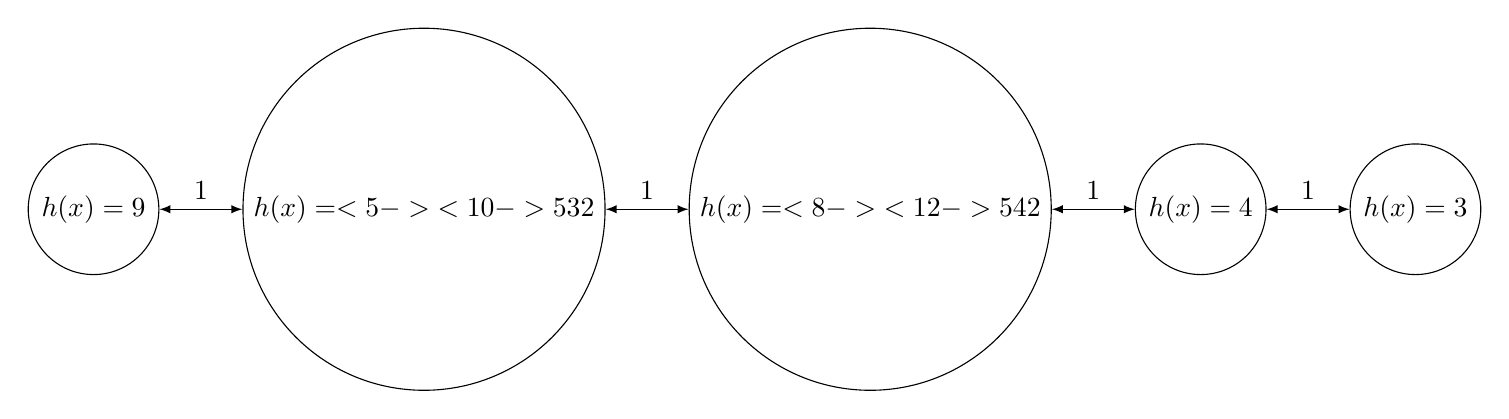
\begin{tikzpicture}[%
state/.style={circle,draw},
action/.style={latex-latex},
weight/.style={auto,swap},
]
\node[state] (1) [visible on={3-}] {$h(x)=9$};
\node[state] (2) [right=3em of 1,filled on={3,7-8}] {$h(x)=\alt<5->{\alt<10->{5}{3}}{2}$}
  edge [action,visible on={3-}]
    node[weight] {1} (1);
\node[state] (3) [right=3em of 2,visible on={3-},filled on={4-6,9-10}] {$h(x)=\alt<8->{\alt<12->{5}{4}}{2}$}
  edge [action,visible on={3-}]
    node[weight] {1} (2);
\node[state] (4) [right=3em of 3,visible on={6-},filled on={11-}] {$h(x)=4$}
  edge [action,visible on={6-}]
    node[weight] {1} (3);
\node[state] (5) [right=3em of 4,visible on={13-}] {$h(x)=3$}
  edge [action,visible on={13-}]
    node[weight] {1} (4);
\end{tikzpicture}
\end{center}
\uncover<14>{Complete in finite, safely explorable environments}
\end{block}
\end{frame}

\part{Key Points}
\begin{frame}{Key Points}
	\begin{block}{Search Algorithms}
		\begin{itemize}
			\item Hill Climbing
			\item Simulated Annealing
			\item Local Beam Search
			\item Discretized Search
			\item Multiple-Belief State Search
			\item LRTA* Search
		\end{itemize}
	\end{block}
\end{frame}

\end{document}


